\chapter{Analyse et sp\'ecification des besoins}
\section{Introduction}
Ce chapitre est consacr\'e \`a l'analyse et \`a la sp\'ecification des besoins fonctionnels et non fonctionnels de la solution qui est une \'etape primordiale pour la r\'ealisation de notre projet.
\section{Analyse des besoins}
Dans cette partie, nous pr\'esenterons les besoins fonctionnels et non fonctionnels identifi\'es apr\`es la s\'election des besoins.
\subsection{Identification des acteurs}
Dans le cas de notre projet on consid\`ere trois acteurs :
\begin{itemize}
\item \textbf{Le prospecteur} : Il a comme mission principale de g\'erer les anomalies de la plateforme.
\item \textbf{L'exploitant} : Il permet de r\'epondre sur les anomalies qui ne sont pas encore r\'esolu.
\item \textbf{L'administrateur} : Il permet de g\'erer les  autres utilisateurs (prospecteurs, exploitants), les machines ,les g\'eolocalisation ... .
\end{itemize}
\subsection{Les besoins fonctionnels}
Au cours de cette \'etape, nous allons extraire les diff\'erentes fonctionnalit\'es offertes par notre projet.
\begin{itemize}
\item L'application \textcolor{red}{prospektor} doit permettre \`a chaque prospecteur de :
\begin{itemize}
\item suivre et consulter les anomalies qui a cr\'eer.
\item consulter la liste des attachements li\'ees par anomalies.
\end{itemize}
\item L'application \textcolor{red}{prospektor} doit permettre \`a chaque exploitant de :
\begin{itemize}
\item suivre et consulter les anomalies par \'etape, date \& criticit\'e.
\item consulter les attachements li\'ees par anomalies.
\item Ajouter des attachements aux anomalies qui ne sont pas encore r\'esolu.
\end{itemize}  
\item L'application \textcolor{red}{prospektor} doit permettre \`a chaque administrateur de :
\begin{itemize}
\item G\'erer :
\begin{itemize}
\item Prospecteurs
\item Exploitants
\item G\'eolocalisation (Mine, Zone, Tranch\'ee, Sortie)
\item Machines
\end{itemize}
\item Consulter :
\begin{itemize}
\item Tourn\'ees
\item Chantiers
\item Erreurs
\item ...
\end{itemize}

\end{itemize} 
 
\end{itemize}

\subsection{Les besoins non fonctionnels}
Outre les fonctions cit\'ees ci-dessus, l'application doit assurer en certaine mesure les caract\'eristiques suivantes :
\begin{itemize}
\item L'efficacit\'e : L'efficacit\'e de l'application doit permettre l'accomplissement de la t\^ache avec le minimum de manipulation. Ceci doit \^etre garanti pour que l'application puisse s'int\'egrer facilement dans l'environnement ou elle va \^etre d\'eploy\'ee.

\item La s\'ecurit\'e : Les diff\'erents comptes utilis\'es par les utilisateurs doivent \^etre s\'ecuris\'es et v\'erifi\'es pour \'eviter les faux comptes et les fausses informations.

\item La fiabilit\'e : Touche \`a l'aspect qualit\'e des donn\'ees et persistance des informations dans l'application ainsi que la vitesse de chargement des interfaces.
\item La performance : le temps de r\'eponse de la plateforme doit \^etre rapide.

\item La maintenabilit\'e : La solution doit \^etre stable face aux changements, ainsi qu'un fort niveau de testabilit\'e assur\'e par les tests fonctionnels.

\item La scalabilit\'e : la solution doit d'\^etre extensible en termes de la charge des requ\^etes trait\'ees.

\item L'\'evolutivit\'e : possibilit\'e d'ajout des nouvelles fonctionnalit\'es au cours du temps selon le besoin des fournisseurs.

\item Le d\'eploiement intelligent: l'introduction des nouveaux changements ne doit pas impacter les modules existants, d'o\`u le besoin d'une d\'emarche de d\'eploiement intelligente de chaque module.

\item La portabilit\'e: facilit\'e de passage d'un environnement de d\'eveloppement et tests vers un environnement de pr\'e-production ou un environnement de production.
\end{itemize} 


\subsection{Diagramme des cas d'utilisation}
Cette figure repr\'esente le diagramme de cas d'utilisation globale de l'acteur prospecteur :
\begin{figure}[H]
	\center{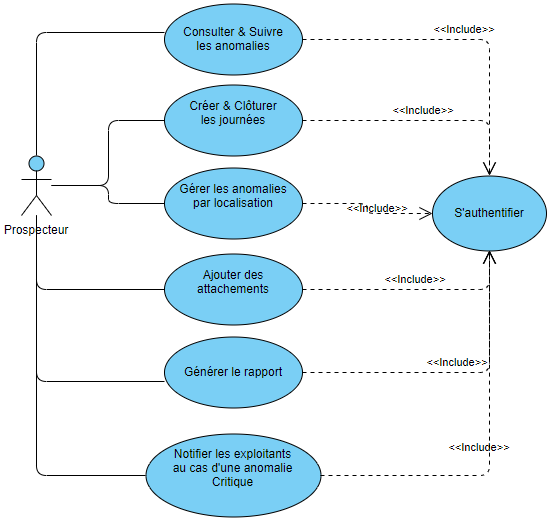
\includegraphics[width=\textwidth]{Figures/prospectorDiagram.png}}
	\caption{\label{fig:my-label} Diagramme de cas d'utilisation globale pour le prospecteur}
\end{figure}

Cette figure repr\'esente le diagramme de cas d'utilisation globale de l'acteur exploitant :
\begin{figure}[H]
	\center{\includegraphics[width=\textwidth]{Figures/exploitantDiagram.png}}
	\caption{\label{fig:my-label} Diagramme de cas d'utilisation globale pour l'exploitant}
\end{figure}

Cette figure repr\'esente le diagramme de cas d'utilisation globale de l'acteur administrateur :
\begin{figure}[H]
	\center{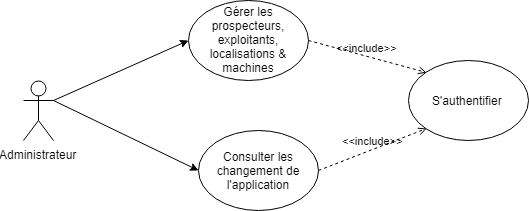
\includegraphics[width=\textwidth]{Figures/adminDiagram.png}}
	\caption{\label{fig:my-label} Diagramme de cas d'utilisation globale pour l'administrateur}
\end{figure}

\subsection{Description des cas d'utilisation}
\textbf{Prospecteur :} Les grandes \'etapes pour un prospecteur lors de l'utilisation de l'application prospektor.
\begin{itemize}
  \item Ouvrir l'application mobile prospektor
  \item S'authentifier
  \begin{itemize}
    \item Consulter les anomalies en cours de traitement
    \item Consulter les demandes d'intervention
    \item Consulter l'historique des anomalies
    \item Consulter le rapport des tourn\'ees
    \item D\'emarrer \& Continuer une tourn\'ee
    \begin{itemize}
      \item sp\'ecifier la localisation du prospection
      \item Remplir la check-list des \'el\'ements \`a auditer
      \item Cr\'eation d'une anomalie au cas d'un d\'erangement
      \item Ajouter des attachements (audio \& photos) si n\'ecessaire
    \end{itemize}
    \item Continuer la tourn\'ee vers un autre chantier
    \item Obtenir le rapport complet de la tourn\'ee 
  \end{itemize}
\end{itemize}

\textbf{Exploitant :} Les grandes \'etapes pour un exploitant lors de l'utilisation de l'application prospektor.
\begin{itemize}
  \item Ouvrir l'application mobile prospektor
  \item S'authentifier
  \begin{itemize}
    \item Consulter les anomalies en cours
    \item Consulter les anomalies \`a traiter
    \item Consulter l'historique des anomalies
  \end{itemize}
\end{itemize}

\textbf{Administrateur :} Les grandes \'etapes pour un administrateur lors de l'utilisation de l'application prospektor.
\begin{itemize}
  \item Ouvrir l'application web prospektor
  \item S'authentifier
  \begin{itemize}
    \item Consulter les utilisateurs (prospecteur \& exploitant).
    \begin{itemize}
    \item Ajouter un utilisateur.
    \item Supprimer un utilisateur.
    \item Modifier un utilisateur.
    \item D\'esactiv\'e un utilisateur.
    \item Consulter les d\'etails d'un utilisateur.
    \end{itemize}
    \item G\'erer les localisations (Mine, Zone, Tranch\'ee, Sortie).
    \item Consulter les machines.
    \begin{itemize}
    \item Ajouter une machine.
    \item Supprimer une machine.
    \item Modifier une machine.
    \item D\'esactiv\'e une machine.
    \item Consulter les d\'etails d'une machine.
    \end{itemize}
    \item Consulter les tourn\'ees.
    \item Consulter les chantiers par zones ou par \'etape.
    \item Consulter les anomalies par criticit\'e.
    \item ...

  \end{itemize}
\end{itemize}

\subsection{Exceptions des cas d'utilisation}

\textbf{Prospecteur :} Les exceptions pour un prospecteur lors de l'utilisation de l'application prospektor:
\begin{itemize}
\item Email ou mot de passe sont incorrecte.
\item Cr\'eer une anomalie sans pr\'eciser leur localisation.
\item Cr\'eer une anomalie sans description.
\item G\'en\'erer le rapport sans terminer toutes les chantiers.
\item ...
\end{itemize}
\textbf{Exploitant :} Les exceptions pour un exploitant lors de l'utilisation de l'application prospektor:
\begin{itemize}
\item Email ou mot de passe sont incorrecte.
\item Repondre \`a une anomalie sans description.
\item Repondre \`a une anomalie d\'ej\`a cl\^oturer.
\item ...
\end{itemize}
\textbf{Administrateur :} Les exceptions pour un administrateur lors de l'utilisation de l'application prospektor:
\begin{itemize}
\item Email ou mot de passe sont incorrecte
\item Ajouter un utilisateur qui n'existe pas dans le group ocp
\item Ajouter une machine sans preciser leur localisation
\item ...
\end{itemize}

\section{Planning du projet}
On a dr\'esse le RoadMap qui va \^etre r\'ealiser entre Mars et Juin sur deux parties. Chaque partie va prendre 8 semaines de travail.

Pour notre projet prospektor, On a d\'efinie 
\begin{itemize}
\item 1 Sprint = 1 Semaine
\item Daily Meeting \& check \`a 10:00 AM
\item Sprint planning chaque mercredi matin
\end{itemize}

\subsection{\gls{MVP}}
\begin{figure}[H]
	\center{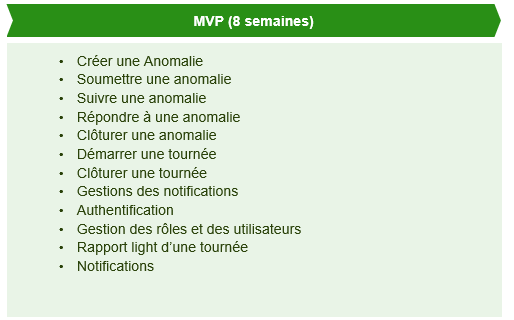
\includegraphics[width=\textwidth]{Figures/mvp.PNG}}
	\caption{\label{fig:my-label} RoadMap de la version \gls{MVP}}
\end{figure}
\subsection{Post MVP}
\begin{figure}[H]
	\center{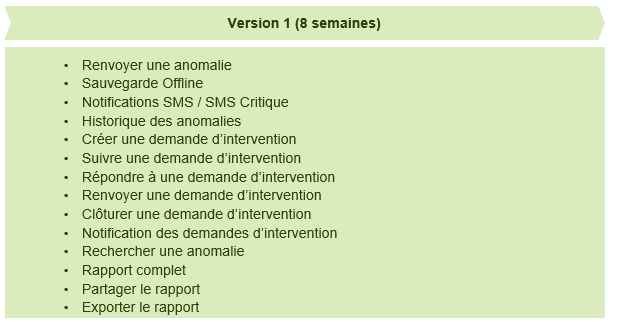
\includegraphics[width=\textwidth]{Figures/version1.PNG}}
	\caption{\label{fig:my-label} RoadMap de la version Post MVP}
\end{figure}

 
\section{Conclusion}
Dans ce chapitre nous avons d\'etect\'e des besoins fonctionnels et non fonctionnels qui sont un compl\'ement de l'existant. Par la suite nous avons pouss\'e l'analyse des besoins vers les diagrammes de cas d'utilisation afin de visualiser les diff\'erentes fonctionnalit\'es de la solution.